\documentclass{article}
\usepackage[yyyymmdd]{datetime}
\usepackage[shortlabels]{enumitem}
\usepackage[nottoc]{tocbibind}
\usepackage{subcaption}
\usepackage{array}
\usepackage{hhline}
\usepackage{multirow}
\usepackage{graphicx}
\graphicspath{{Code/images/}}
\usepackage[margin=1in]{geometry}
\usepackage[dvipsnames]{xcolor}
\usepackage{colortbl}
\usepackage[framemethod=TikZ]{mdframed}
\usepackage{amsfonts}
\usepackage{amsmath}
\usepackage{float}
\usepackage{tikz}
\usepackage{amsthm}
\newtheoremstyle{problemstyle}{3pt}{3pt}{\normalfont}{}{\bfseries}{\normalfont\bfseries:}{.5em}{}
\theoremstyle{problemstyle}
\newmdtheoremenv[
  linewidth=0pt,
  linecolor=RoyalBlue,
  roundcorner=5pt,
  innertopmargin=6pt,
  innerbottommargin=6pt,
  innerleftmargin=6pt,
  innerrightmargin=6pt,
]{problem}{Problem}

% Example
\newmdtheoremenv[
  linewidth=1pt,
  linecolor=ForestGreen,
  backgroundcolor=ForestGreen!10,
  roundcorner=5pt,
  nobreak=true
]{example}{Example}

% Theorem
\newmdtheoremenv[
  linewidth=1pt,
  linecolor=BrickRed,
  backgroundcolor=BrickRed!10,
  roundcorner=5pt,
  nobreak=true
]{theorem}{Theorem}

% Remark
\newmdtheoremenv[
  linewidth=1pt,
  linecolor=Goldenrod,
  backgroundcolor=Goldenrod!10,
  roundcorner=5pt,
  nobreak=true
]{remark}{Remark}

% Solution
\newenvironment{solution}[2]{%
  \begin{mdframed}[linewidth=0.8pt,linecolor=Gray,backgroundcolor=Gray!5,roundcorner=5pt, nobreak=#2]%
    \noindent\textbf{Solution\if\relax\detokenize{#1}\relax\else~(#1)\fi.}%
}{%
\hfill $ \diamond $ 
  \end{mdframed}%
}

\usepackage{listings}

\lstset{breaklines=true}
\definecolor{vscode-blue}{RGB}{64, 116, 160}   % Keywords
\definecolor{vscode-green}{RGB}{95, 203, 114}   % Strings
\definecolor{vscode-gray}{RGB}{128, 128, 128}   % Comments
\definecolor{vscode-orange}{RGB}{206, 145, 120} % Numbers/Constants
\definecolor{vscode-purple}{RGB}{204, 124, 255} % Functions/Types
\definecolor{vscode-cyan}{RGB}{155, 199, 217}   % Preprocessor

\lstdefinestyle{visual-studio}{
    language=C,
    backgroundcolor=\color{Gray!5},
    commentstyle=\color{vscode-gray}\ttfamily,
    keywordstyle=\color{vscode-blue}\ttfamily,
    stringstyle=\color{vscode-green}\ttfamily,
    numberstyle=\color{vscode-orange}\ttfamily,
    identifierstyle=\color{black}\ttfamily,
    breaklines=true,
    showstringspaces=false,
    tabsize=4,
    % Additional settings for more Visual Studio feel
    emph=[1]{void, int, double, float, char, bool, short, long, signed, unsigned, class, struct, enum, union, typedef, template}, % Common types
    emphstyle=[1]\color{vscode-purple},
    emph=[2]{printf, scanf, cin, cout, return, new, delete, if, else, while, do, for, switch, case, default, break, continue, goto, throw, try, catch, const, static, extern, volatile, register, restrict, inline, explicit, virtual, friend, namespace, using, private, protected, public, operator}, % Standard keywords
    emphstyle=[2]\color{vscode-blue},
            keywordstyle=[2]\color{vscode-cyan}\ttfamily\bfseries,
    morekeywords={\#include, \#define, \#ifdef, \#ifndef, \#endif, \#pragma},
    basicstyle=\small
}


% Make header with name and date etc.
\usepackage{fancyhdr}
\lhead{Pedro D. Llerenas\\Programaci\'on y Algoritmos I}
\rhead{\today\\Tarea III}
\thispagestyle{fancy}

\usepackage[utf8]{inputenc}
\setlength{\parindent}{0pt} % Don't indent new paragraphs
\setlength{\headheight}{24pt} 

\newcommand{\Z}{\mathbb Z}
\newcommand{\Q}{\mathbb Q}
\newcommand{\R}{\mathbb R}
\newcommand{\C}{\mathbb C}
\newcommand{\N}{\mathbb N}


\begin{document}
\begin{problem}
(25\%) Implemente las siguientes operaciones (como funciones) para el procesamiento digital de im\'agenes:
\begin{enumerate}[a)]
	\item Filtro de la \textbf{Media}: 
    Primero, para compilar este programa, usar


    \texttt{gcc pgm\_io.c kernel\_io.c convolution.c compare.c p1.c -o p1}.

    Para el filtro de la media, usar

    \texttt{./p1 images/<input-file> images/<output-file> mean <window-dimension>}
	      \begin{enumerate}[i)]
		      \item Ventana de $ 3\times 3 $
		            \begin{figure}[H]
			            \begin{subfigure}{.45\textwidth}
				            \centering
				            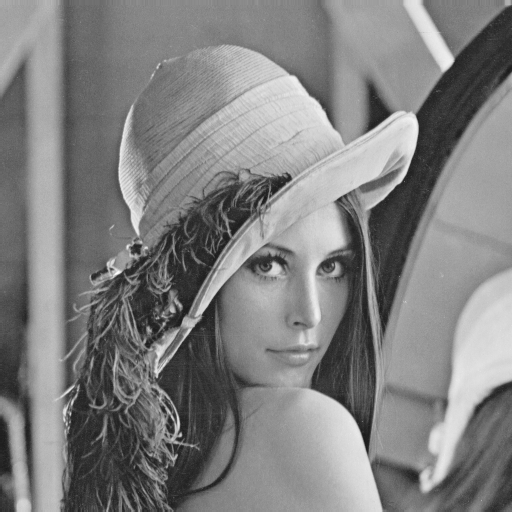
\includegraphics[width=0.95\textwidth]{lena_ascii.png}
				            \caption{Original image of Lena.}
			            \end{subfigure}
			            \hfill
			            \begin{subfigure}{.45\textwidth}
				            \centering
				            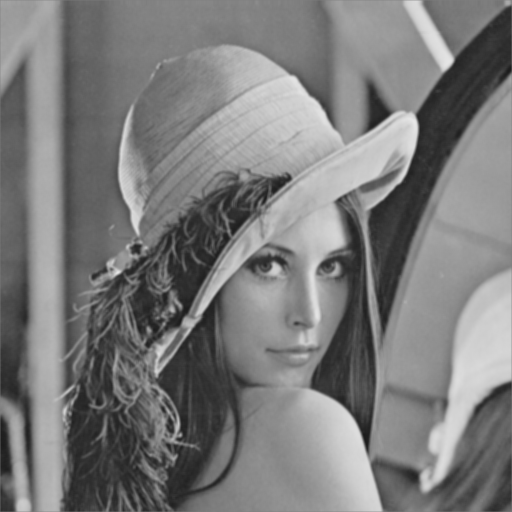
\includegraphics[width=0.95\textwidth]{lena_mean_3x3.png}
				            \caption{$ 3\times 3 $ mean filter applied to Lena.}
				            \label{fig:lena_mean_3x3}
			            \end{subfigure}
			            \caption{Comparison of original and $ 3\times 3 $ mean filtered images.}
		            \end{figure}
		      \item Ventana de $ 5\times 5 $.
		            \begin{figure}[H]
			            \begin{subfigure}{.45\textwidth}
				            \centering
				            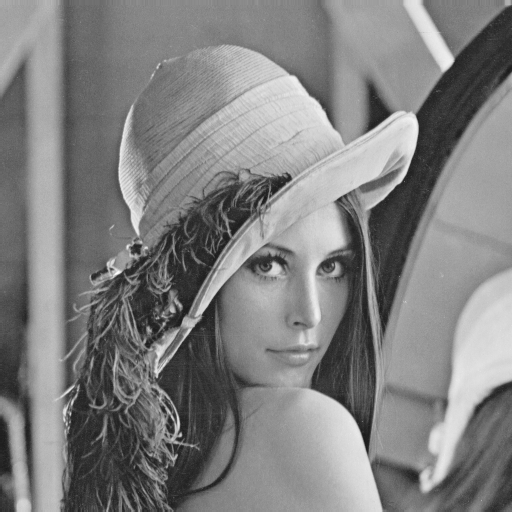
\includegraphics[width=0.95\textwidth]{lena_ascii.png}
				            \caption{Original image of Lena.}
			            \end{subfigure}
			            \hfill
			            \begin{subfigure}{.45\textwidth}
				            \centering
				            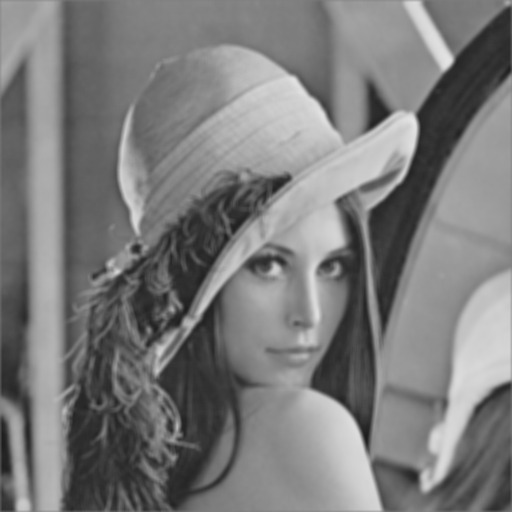
\includegraphics[width=0.95\textwidth]{lena_mean_5x5.png}
				            \caption{$ 5\times 5 $ mean filter applied to Lena.}
				            \label{fig:lena_mean_5x5}
			            \end{subfigure}
			            \caption{Comparison of original and $ 5\times 5 $ mean filtered images.}
		            \end{figure}

		      \item Ventana de $ 7\times 7 $.
		            \begin{figure}[H]
			            \begin{subfigure}{.45\textwidth}
				            \centering
				            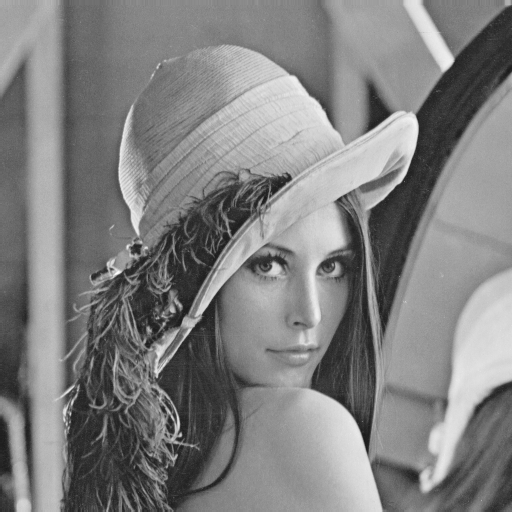
\includegraphics[width=0.95\textwidth]{lena_ascii.png}
				            \caption{Original image of Lena.}
			            \end{subfigure}
			            \hfill
			            \begin{subfigure}{.45\textwidth}
				            \centering
				            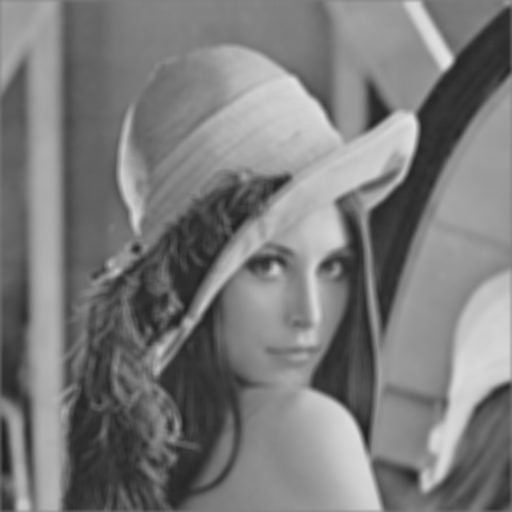
\includegraphics[width=0.95\textwidth]{lena_mean_7x7.png}
				            \caption{$ 7\times 7 $ mean filter applied to Lena.}
				            \label{fig:lena_mean_7x7}
			            \end{subfigure}
			            \caption{Comparison of original and $ 7\times 7 $ mean filtered images.}
		            \end{figure}
	      \end{enumerate}

	\item Filtro de la \textbf{Mediana}:

    Para el filtro de la mediana, usar:

    \texttt{./p1 images/<input-file> images/<output-file> median <window-dimension>}
	      \begin{enumerate}[i)]
		      \item Ventana de $ 3\times 3 $.
		            \begin{figure}[H]
			            \begin{subfigure}{.45\textwidth}
				            \centering
				            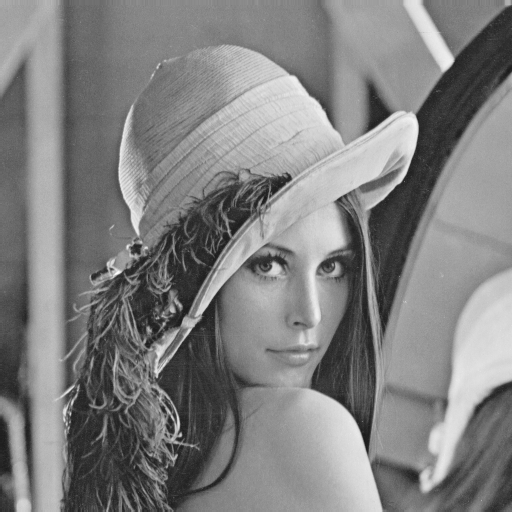
\includegraphics[width=0.95\textwidth]{lena_ascii.png}
				            \caption{Original image of Lena.}
			            \end{subfigure}
			            \hfill
			            \begin{subfigure}{.45\textwidth}
				            \centering
				            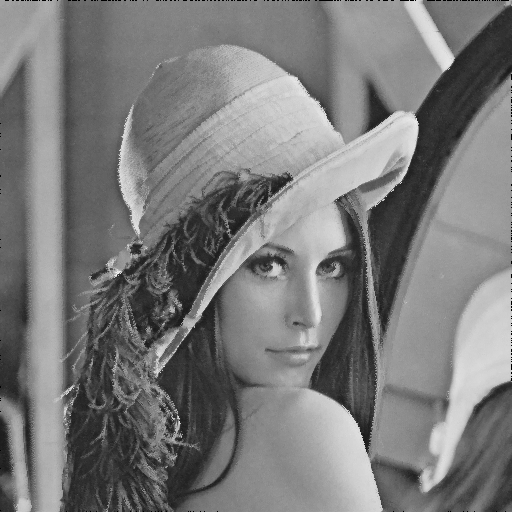
\includegraphics[width=0.95\textwidth]{lena_median_3x3.png}
				            \caption{$ 3\times 3 $ median filter applied to Lena.}
				            \label{fig:lena_median_3x3}
			            \end{subfigure}
			            \caption{Comparison of original and $ 3\times 3 $ median filtered images.}
		            \end{figure}

		      \item Ventana de $ 5\times 5 $.
		            \begin{figure}[H]
			            \begin{subfigure}{.45\textwidth}
				            \centering
				            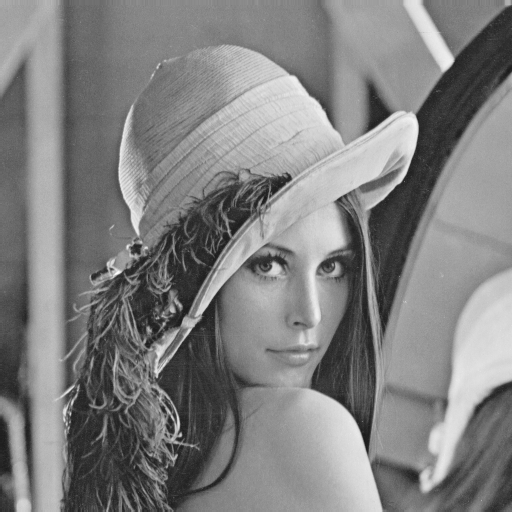
\includegraphics[width=0.95\textwidth]{lena_ascii.png}
				            \caption{Original image of Lena.}
			            \end{subfigure}
			            \hfill
			            \begin{subfigure}{.45\textwidth}
				            \centering
				            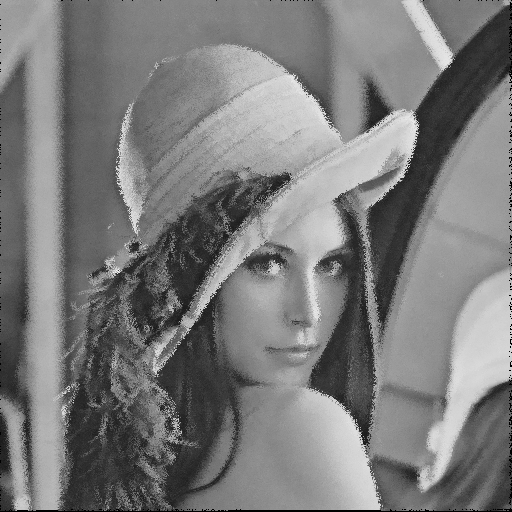
\includegraphics[width=0.95\textwidth]{lena_median_5x5.png}
				            \caption{$5\times 5$ median filter applied to Lena.}
				            \label{fig:lena_median_5x5}
			            \end{subfigure}
			            \caption{Comparison of original and $ 5\times 5 $ median filtered images.}
		            \end{figure}

		      \item Ventana de $ 7\times 7 $.
		            \begin{figure}[H]
			            \begin{subfigure}{.45\textwidth}
				            \centering
				            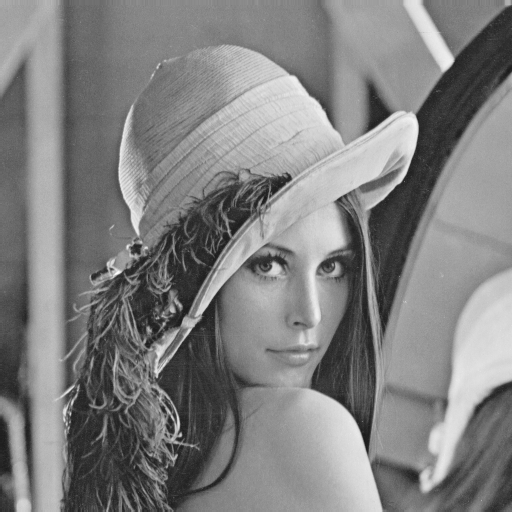
\includegraphics[width=0.95\textwidth]{lena_ascii.png}
				            \caption{Original image of Lena.}
			            \end{subfigure}
			            \hfill
			            \begin{subfigure}{.45\textwidth}
				            \centering
				            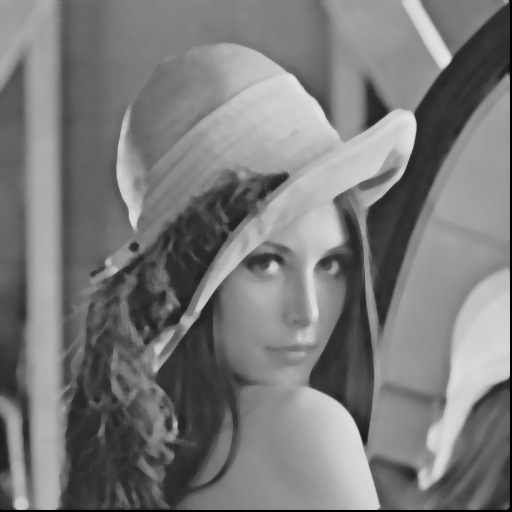
\includegraphics[width=0.95\textwidth]{lena_median_7x7.png}
				            \caption{$ 7\times 7 $ median filter applied to Lena.}
				            \label{fig:lena_median_7x7}
			            \end{subfigure}
			            \caption{Comparison of original and $ 7\times 7 $ median filtered images.}
		            \end{figure}
	      \end{enumerate}
	\item Filtro \textbf{Gaussiano}:
    
    Para el filtro de la mediana, usar:

    \texttt{./p1 images/<input-file> images/<output-file> gaussian <window-dimension>}
	      \begin{enumerate}[i)]
		      \item Ventana de $ 3\times 3 $.


		            \begin{figure}[H]
			            \begin{subfigure}{.45\textwidth}
				            \centering
				            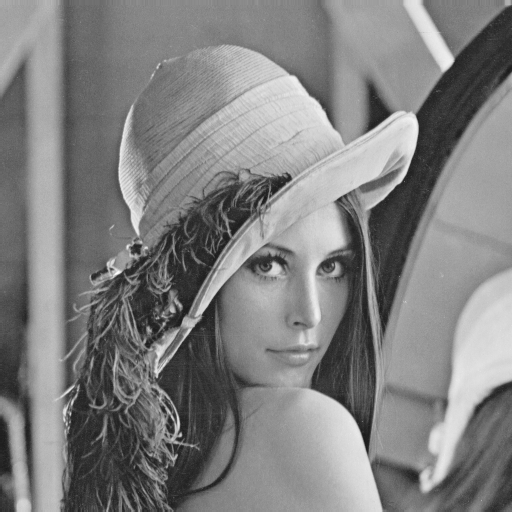
\includegraphics[width=0.95\textwidth]{lena_ascii.png}
				            \caption{Original image of Lena.}
			            \end{subfigure}
			            \hfill
			            \begin{subfigure}{.45\textwidth}
				            \centering
				            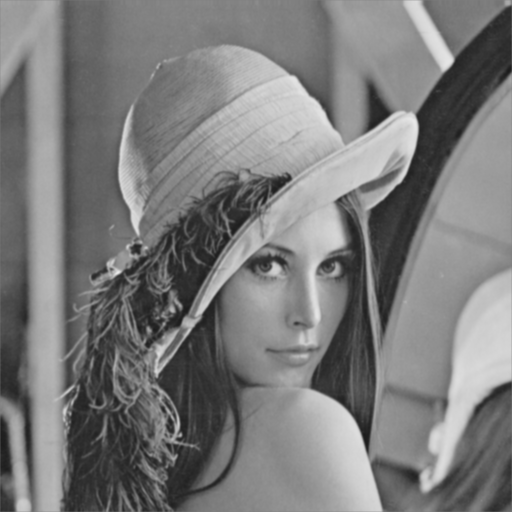
\includegraphics[width=0.95\textwidth]{lena_gaussian_3x3.png}
				            \caption{$ 3\times 3 $ Gaussian filter applied to Lena.}
				            \label{fig:lena_Gaussian_3x3}
			            \end{subfigure}
			            \caption{Comparison of original and $ 3\times 3 $ Gaussian filtered images.}
		            \end{figure}
		      \item Ventana de $ 5\times 5 $.
		            \begin{figure}[H]
			            \begin{subfigure}{.45\textwidth}
				            \centering
				            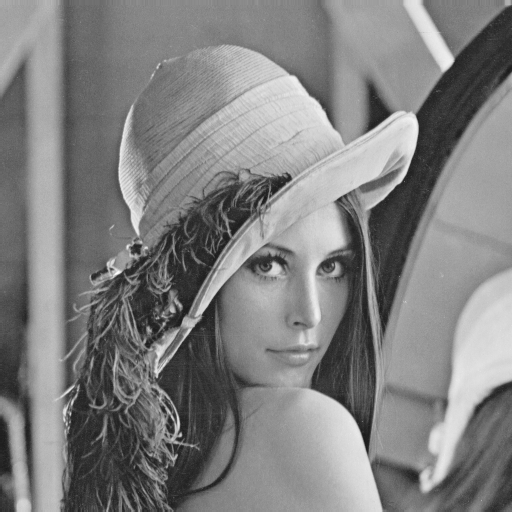
\includegraphics[width=0.95\textwidth]{lena_ascii.png}
				            \caption{Original image of Lena.}
			            \end{subfigure}
			            \hfill
			            \begin{subfigure}{.45\textwidth}
				            \centering
				            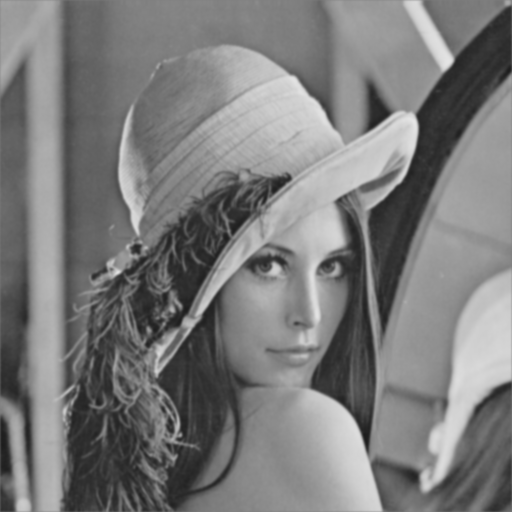
\includegraphics[width=0.95\textwidth]{lena_gaussian_5x5.png}
				            \caption{$ 5\times 5 $ Gaussian filter applied to Lena.}
				            \label{fig:lena_Gaussian_5x5}
			            \end{subfigure}
			            \caption{Comparison of original and $ 5\times 5 $ Gaussian filtered images.}
		            \end{figure}
		      \item Ventana de $ 7\times 7 $.
		            \begin{figure}[H]
			            \begin{subfigure}{.45\textwidth}
				            \centering
				            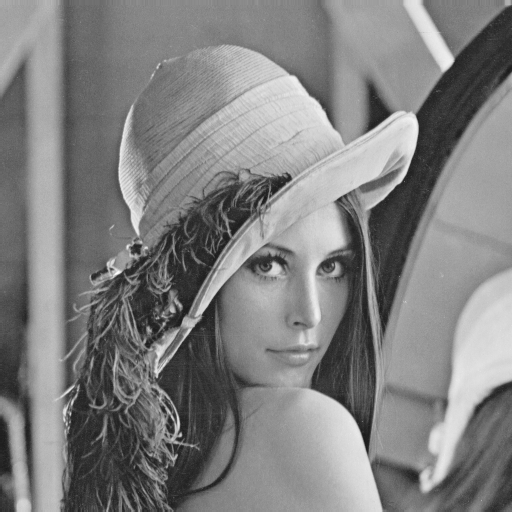
\includegraphics[width=0.95\textwidth]{lena_ascii.png}
				            \caption{Original image of Lena.}
			            \end{subfigure}
			            \hfill
			            \begin{subfigure}{.45\textwidth}
				            \centering
				            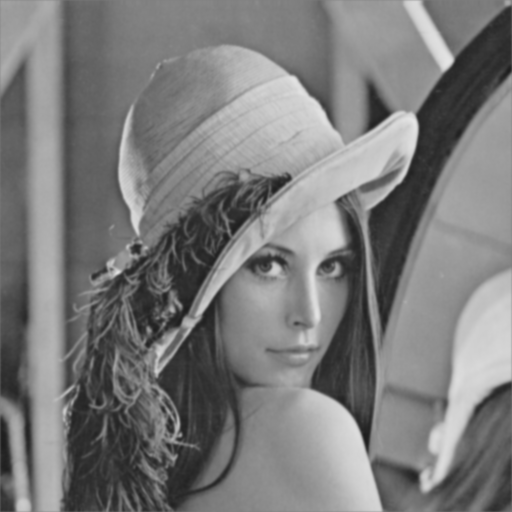
\includegraphics[width=0.95\textwidth]{lena_gaussian_7x7.png}
				            \caption{$ 7\times 7 $ Gaussian filter applied to Lena.}
				            \label{fig:lena_Gaussian_7x7}
			            \end{subfigure}
			            \caption{Comparison of original and $ 7\times 7 $ Gaussian filtered images.}
		            \end{figure}
	      \end{enumerate}
\end{enumerate}
\end{problem}

\begin{problem}
(25\%) Funci\'on que calcule la derivada de $ I_{M\times N} $ usando las siguientes definiciones:
\begin{enumerate}[a)]
	\item Aproximaci\'on a la magnitud del gradiente:
	      \begin{align*}
		      \lVert G(f(x,y))\rVert \approx \lVert G_x\rVert + \lVert G_y\rVert \cong \lvert f[i,j] - f[i+1,j] \rvert + \lvert f[i, j+1] - f[i,j]\rvert
	      \end{align*}
        Para compilar el progrma, usar 

\texttt{gcc pgm\_io.c kernel\_io.c convolution.c compare.c p2.c -o p2}.

Para usar el filtro del gradiente, usar


\texttt{./p2 images/<input-file> images/<output-file> gradient}.
	      \begin{figure}[H]
		      \begin{subfigure}{.45\textwidth}
			      \centering
			      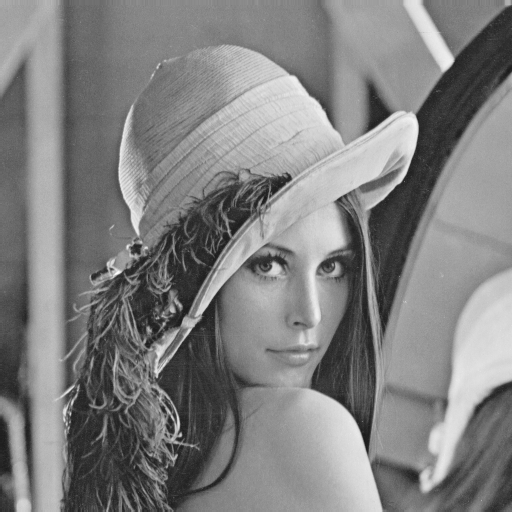
\includegraphics[width=0.95\textwidth]{lena_ascii.png}
			      \caption{Original image of Lena.}
		      \end{subfigure}
		      \hfill
		      \begin{subfigure}{.45\textwidth}
			      \centering
			      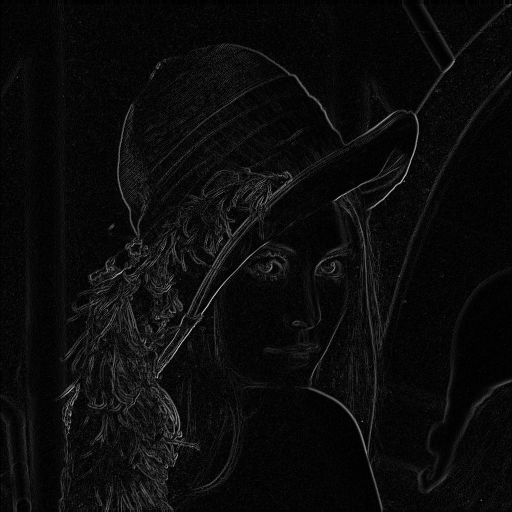
\includegraphics[width=0.95\textwidth]{lena_gradient.png}
			      \caption{Gradient magnitude filter applied to Lena.}
			      \label{fig:lena_gradient}
		      \end{subfigure}
		      \caption{Comparison of original and gradient filtered images.}
	      \end{figure}

	\item Aproximaci\'on a la magnitud de los operadores de \textbf{Scharr}:
	      \begin{align*}
		      \mathbf{S}_{H} =
		      \begin{bmatrix}
			      3  & 0 & -3  \\
			      10 & 0 & -10 \\
			      3  & 0 & -3
		      \end{bmatrix},
		      \qquad \mathbf{S}_{V} =
		      \begin{bmatrix}
			      3  & 10  & 3  \\
			      0  & 0   & 0  \\
			      -3 & -10 & -3
		      \end{bmatrix}.
	      \end{align*}
Para usar el filtro de Scharr, usar


\texttt{./p2 images/<input-file> images/<output-file> scharr}.

	      \begin{figure}[H]
		      \begin{subfigure}{.45\textwidth}
			      \centering
			      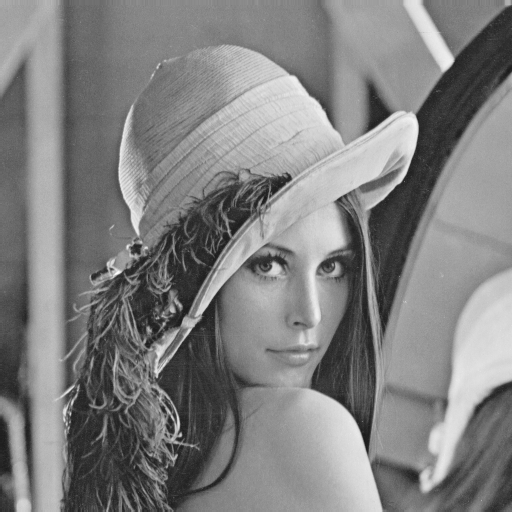
\includegraphics[width=0.95\textwidth]{lena_ascii.png}
			      \caption{Original image of Lena.}
		      \end{subfigure}
		      \hfill
		      \begin{subfigure}{.45\textwidth}
			      \centering
			      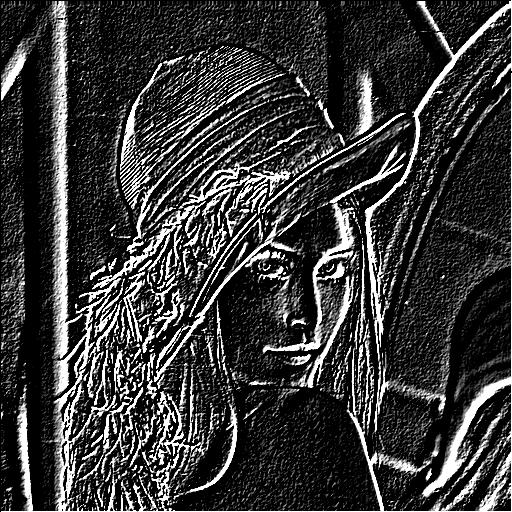
\includegraphics[width=0.95\textwidth]{lena_scharr.png}
			      \caption{Scharr filter applied to Lena.}
			      \label{fig:lena_scharr}
		      \end{subfigure}
		      \caption{Comparison of original and Scharr filtered images.}
	      \end{figure}
	\item Aproximaci\'on a la maginitud del operador \textbf{Laplaciano} positivo:
	      \begin{align*}
		      \mathbf{H}_{1} = \begin{bmatrix}
			                       0 & 1  & 0 \\
			                       1 & -4 & 1 \\
			                       0 & 1  & 0 \\
		                       \end{bmatrix},
		      \qquad
		      \mathbf{H}_{2} = \begin{bmatrix}
			                       1 & 4   & 1 \\
			                       4 & -20 & 4 \\
			                       1 & 4   & 1 \\
		                       \end{bmatrix}.
	      \end{align*}
Para usar el filtro Laplaciano $ \mathbf{H}_1 $, usar


\texttt{./p2 images/<input-file> images/<output-file> laplacian4}.
	      \begin{figure}[H]
		      \begin{subfigure}{.45\textwidth}
			      \centering
			      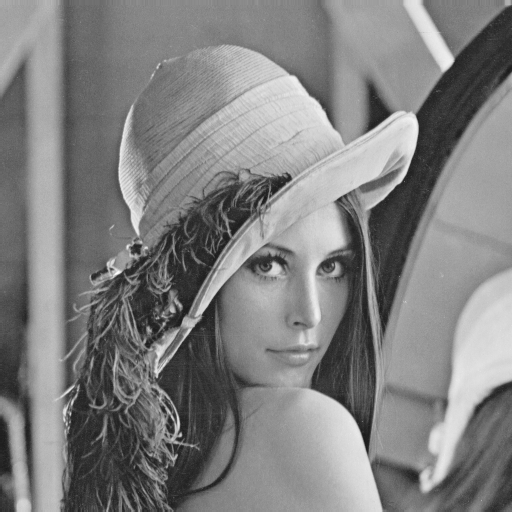
\includegraphics[width=0.95\textwidth]{lena_ascii.png}
			      \caption{Original image of Lena.}
		      \end{subfigure}
		      \hfill
		      \begin{subfigure}{.45\textwidth}
			      \centering
			      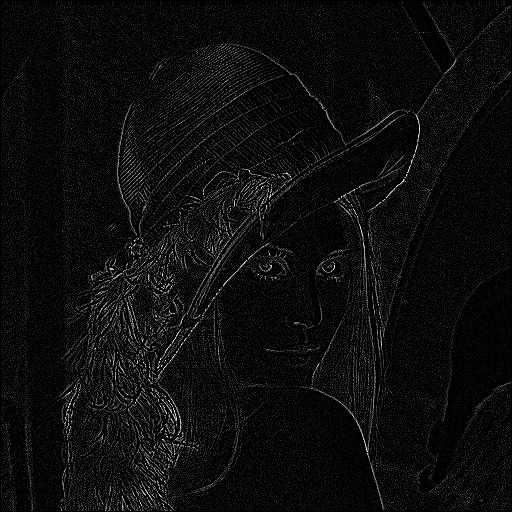
\includegraphics[width=0.95\textwidth]{lena_laplacian4.png}
			      \caption{$ \mathbf{H}_1 $ filter applied to Lena.}
			      \label{fig:lena_laplacian4}
		      \end{subfigure}
		      \caption{Comparison of original and Laplacian filtered images.}
	      \end{figure}
Para usar el filtro Laplaciano $ \mathbf{H}_2 $, usar


\texttt{./p2 images/<input-file> images/<output-file> laplacian20}.

	      \begin{figure}[H]
		      \begin{subfigure}{.45\textwidth}
			      \centering
			      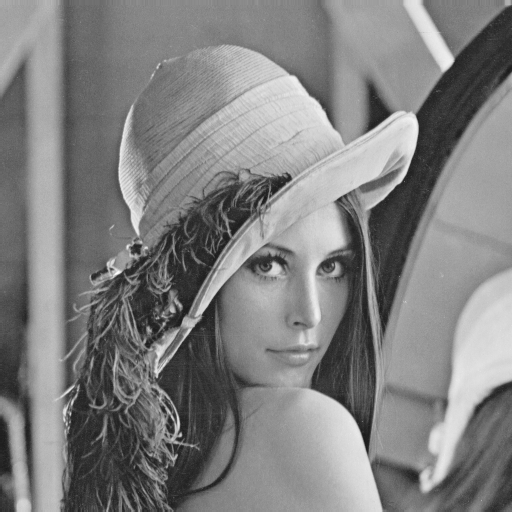
\includegraphics[width=0.95\textwidth]{lena_ascii.png}
			      \caption{Original image of Lena.}
		      \end{subfigure}
		      \hfill
		      \begin{subfigure}{.45\textwidth}
			      \centering
			      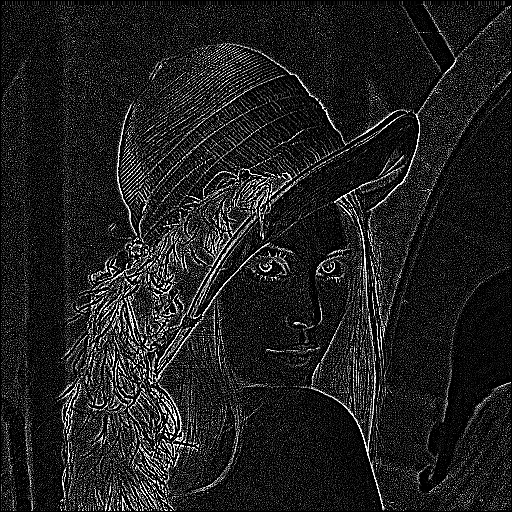
\includegraphics[width=0.95\textwidth]{lena_laplacian20.png}
			      \caption{$ \mathbf{H}_2 $ filter applied to Lena.}
			      \label{fig:lena_laplacian20}
		      \end{subfigure}
		      \caption{Comparison of original and Laplacian filtered images.}
	      \end{figure}
\end{enumerate}
\end{problem}

\begin{problem}
(10\%) Cambiar la representaci\'on del n\'umero de bits de la imagen de entrada. Pedir como entrada la nueva representaci\'on ($ 1\leq \text{bits}< 8 $).

Para compilar este programa, usar

\texttt{gcc pgm\_io.c p3.c -o p3} 

y ejecutar usando 

\texttt{./p3 images/<input-file> images/<output-file> <bits>}.

\begin{figure}[H]
	\begin{subfigure}{.45\textwidth}
		\centering
		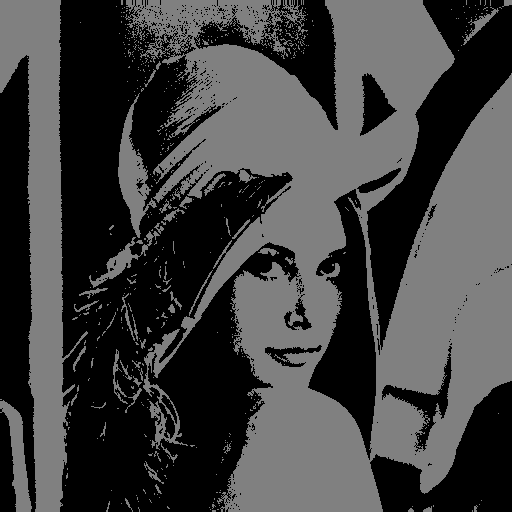
\includegraphics[width=0.95\textwidth]{lena_b1.png}
		\caption{Image of Lena with a 1 bit representation.}
		\label{fig:lena_b1}
	\end{subfigure}
	\hfill
	\begin{subfigure}{.45\textwidth}
		\centering
		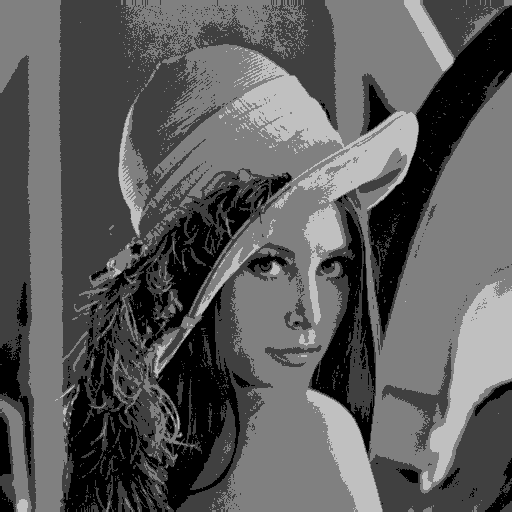
\includegraphics[width=0.95\textwidth]{lena_b2.png}
		\caption{Image of Lena with a 2 bit representation.}
		\label{fig:lena_b2}
	\end{subfigure}
\end{figure}
\begin{figure}[H]
	\begin{subfigure}{.45\textwidth}
		\centering
		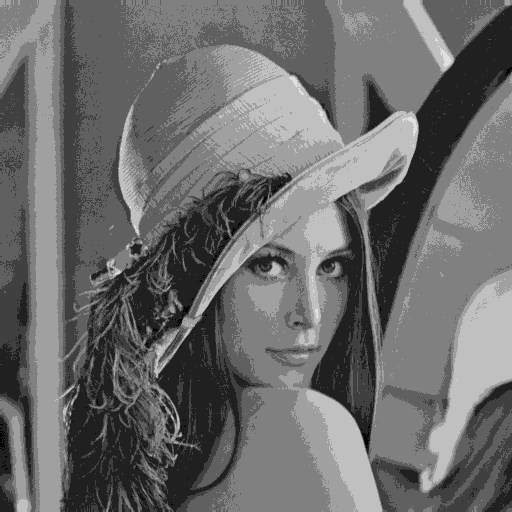
\includegraphics[width=0.95\textwidth]{lena_b3.png}
		\caption{Image of Lena with a 3 bit representation.}
		\label{fig:lena_b3}
	\end{subfigure}
	\hfill
	\begin{subfigure}{.45\textwidth}
		\centering
		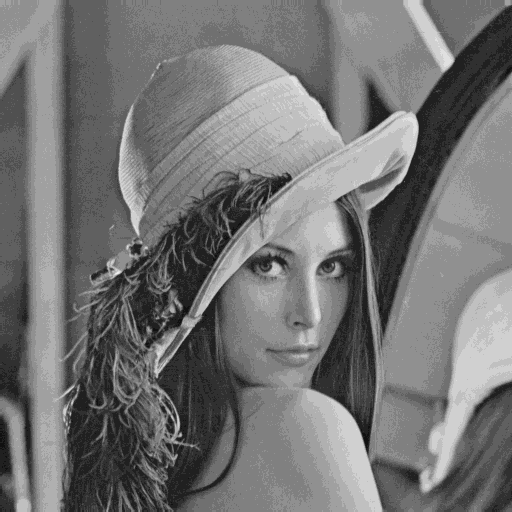
\includegraphics[width=0.95\textwidth]{lena_b4.png}
		\caption{Image of Lena with a 4 bit representation.}
		\label{fig:lena_b4}
	\end{subfigure}
\end{figure}
\begin{figure}[H]
	\begin{subfigure}{.45\textwidth}
		\centering
		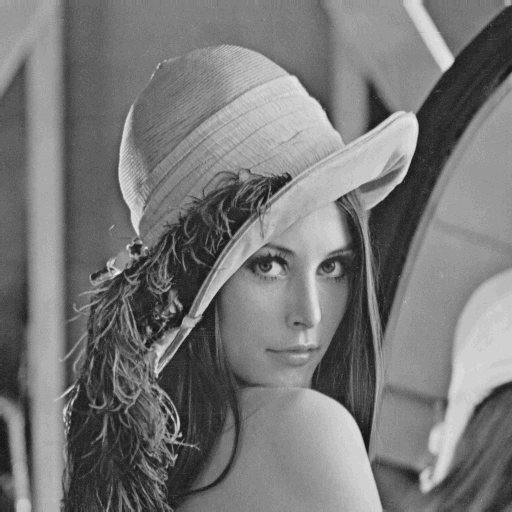
\includegraphics[width=0.95\textwidth]{lena_b5.png}
		\caption{Image of Lena with a 5 bit representation.}
		\label{fig:lena_b5}
	\end{subfigure}
	\hfill
	\begin{subfigure}{.45\textwidth}
		\centering
		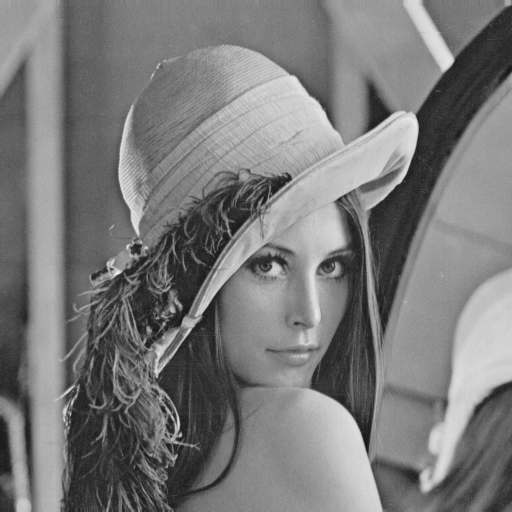
\includegraphics[width=0.95\textwidth]{lena_b6.png}
		\caption{Image of Lena with a 6 bit representation.}
		\label{fig:lena_b6}
	\end{subfigure}
\end{figure}
\begin{figure}[H]
	\begin{subfigure}{.45\textwidth}
		\centering
		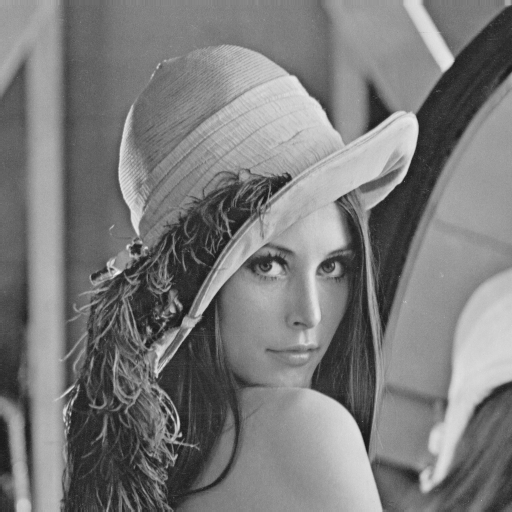
\includegraphics[width=0.95\textwidth]{lena_b7.png}
		\caption{Image of Lena with a 7 bit representation.}
		\label{fig:lena_b7}
	\end{subfigure}
	\hfill
	\begin{subfigure}{.45\textwidth}
		\centering
		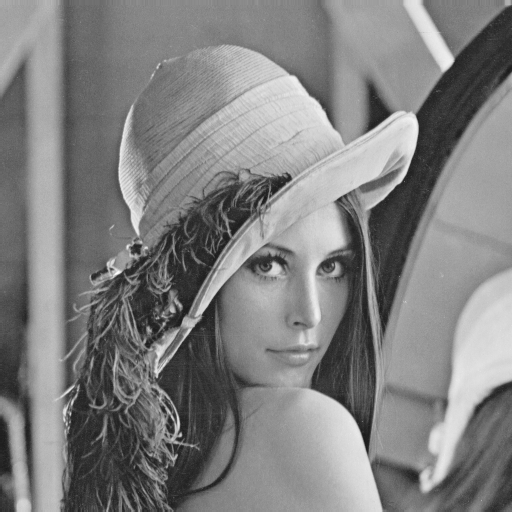
\includegraphics[width=0.95\textwidth]{lena_ascii.png}
		\caption{Original image (8 bits).}
	\end{subfigure}
\end{figure}
\end{problem}

\begin{problem}
(20\%) Programa que sume, reste y multiplique $4 \leq N \leq 8$ matrices cuadradas $ M\times M $ usando arreglos en 3 dimensiones. Escribir funciones para leer la matriz y para cada una de las operaciones con las $ N $ matrices (argumentos variables). Preguntar los valores de $ N $ y $ M $. Usar memoria din\'amica y apuntadores en el recorrido de las matrices.


Para compilar y ejecutar, usar \texttt{gcc p4.c -o p4} y ejecutar usando \texttt{./p4 <M> <N>}.
\end{problem}

\begin{problem}
(20\%) Programa que lea un archivo de texto y despliegue la siguiente información:
\begin{enumerate}[a.]
	\item Tama\~no en bytes;
	\item N\'umero de l\'ineas;
	\item Probabilidad (Pbb) de aparici\'on de cada una de las letras del alfabeto (no haga diferencia entre min\'usculas y may\'usculas ni acentuadas);
	\item $Pbb(x|y=e)$, para $ x\in \{a,\dots, z, A, \dots, Z\} $


    Para correr el c\'odigo de este problema, usar \texttt{gcc p5.c -o p5} y \texttt{./p5 <archivo>}. El siguiente output es usando \texttt{Don-Quijote-Ingles.txt}:
\begin{center}
  \texttt{File has 2347772 bytes}\\
  \texttt{File has 40007 lines}
\end{center}
	      \begin{table}[H]
		      \centering
		      \begin{tabular}{|l|c|c|c|}
			      \hline
			      \textbf{char} & \textbf{freq.} & \textbf{pbb(char)} & $\mathbf{pbb(char|e)}$ \\
			      \hline
			      a             & 148973         & 0.082683           & 0.052954               \\
			      b             & 25519          & 0.014164           & 0.001034               \\
			      c             & 41228          & 0.022882           & 0.015536               \\
			      d             & 81587          & 0.045283           & 0.072217               \\
			      e             & 219491         & 0.121822           & 0.032457               \\
			      f             & 41740          & 0.023167           & 0.008720               \\
			      g             & 34246          & 0.019007           & 0.004834               \\
			      h             & 125331         & 0.069562           & 0.001449               \\
			      i             & 121892         & 0.067653           & 0.013226               \\
			      j             & 1654           & 0.000918           & 0.000396               \\
			      k             & 12516          & 0.006947           & 0.001048               \\
			      l             & 66773          & 0.037061           & 0.039113               \\
			      m             & 45899          & 0.025475           & 0.020903               \\
			      n             & 124804         & 0.069269           & 0.077666               \\
			      o             & 146904         & 0.081535           & 0.001982               \\
			      p             & 26297          & 0.014595           & 0.010656               \\
			      q             & 4213           & 0.002338           & 0.001394               \\
			      r             & 100117         & 0.055567           & 0.124474               \\
			      s             & 114743         & 0.063685           & 0.064385               \\
			      t             & 169437         & 0.094041           & 0.023122               \\
			      u             & 50147          & 0.027833           & 0.000260               \\
			      v             & 18704          & 0.010381           & 0.013964               \\
			      w             & 40609          & 0.022539           & 0.004356               \\
			      x             & 4562           & 0.002532           & 0.006442               \\
			      y             & 33237          & 0.018447           & 0.016871               \\
			      z             & 1106           & 0.000614           & 0.000547               \\
			      \hline
		      \end{tabular}
		      \caption{Character frequency and probabilities}
		      \label{table:char_data}
	      \end{table}
\end{enumerate}


\end{problem}

\bibliographystyle{plain}
\bibliography{references}

\end{document}
